\chapter{Développement durable}

À l'heure où la France s'inquiète de l'impact écologiques sur la planète des climatiseurs pour refroidir nos pièces durant les fortes chaleurs, ce problème ne semble pas être au coeur des préoccupations par UTP.

Les températures extérieures étant très élevées en Malaisie, tous les batiments (gare, restaurants, hotels, etc.) et les voitures sont équipés de climatiseurs. Cependant le réglages de ces derniers sont souvent bien trop froid ($\approx 20^{\circ}C$) et nous oblige à porter des vetêments chauds et longs à l'interieur des batiments malgré la température extérieure dépassant largement les $30^{\circ}C$ l'ensemble de  notre séjour.

\begin{figure}[h]
  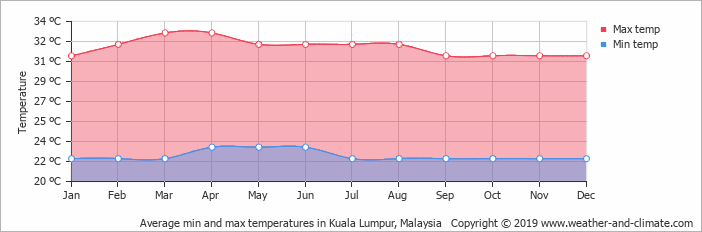
\includegraphics[width=1\linewidth]{content/imgs/temp.png}
  \caption{Temperatures moyennes minimales et maximales en Malaisie, dans la capitale}
  \label{fig:climate}
\end{figure}

Malgré l'usage excessif des climatiseurs, les batiments récents de l'université ne sont pas dotés d'une isolation thermique comparable aux batiments récents construit en France. Pour ne prendre qu'un exemple, je travaillais dans la bibliothèque universitaire, cette dernière possède une immense façade vitrée bordée de portes, elles aussi vitrées, laissant la fraicheur du batiments se faire ressentir sur plusieurs mètres à l'exterieur. De plus les climatiseurs des pièces des laboratoires de l'université restent la plupart du temps allumés toutes la journée malgré l'absence de personne dans les pièces climatisées, et avec les portes ouvertes (qui donnent directement sur l'extérieur).

D'après le site de l'université \cite{utp_gender}, une attention particulière est mise en oeuvre pour favoriser la diversité des genres au sein de l'université, que ce soit au niveau des étudiants, des employés et du personnel pédagogique.
